\section{Experiments}

All of our experiments are run with a limitation of 1mb RAM - a limitation we achieved by using cgroups in linux - on a standard mechanical hard-drive. This was done to significantly reduce the running time of our experiments and the amount of data required. 
During the first part of our testing we did in no way manage to get the expected results. In fact they were more or less opposite of the what the theory predicted. For example running the external merge sort with one small and one large N showed the larger N to be faster! We have not managed to find an adequate explanation for this so far and it would require require more investigation to find the reason.
We have however found a solution to the above problem, which gives results that fit the theory a lot better. By including an optimization flag for our compiler (in our case we used clang) not only did the running time decrease by roughly 1/3 but the results of the test cases also align better with the expected result. 

\subsection{Stream implementations}
The tests for our streams include testing different values of the buffersize b, the amount of streams d, and with a varying number of elements n. 
Each test has been run 100 times where the average is the values used in the graphs. 

\subsubsection{SingleItemStream and FStream}
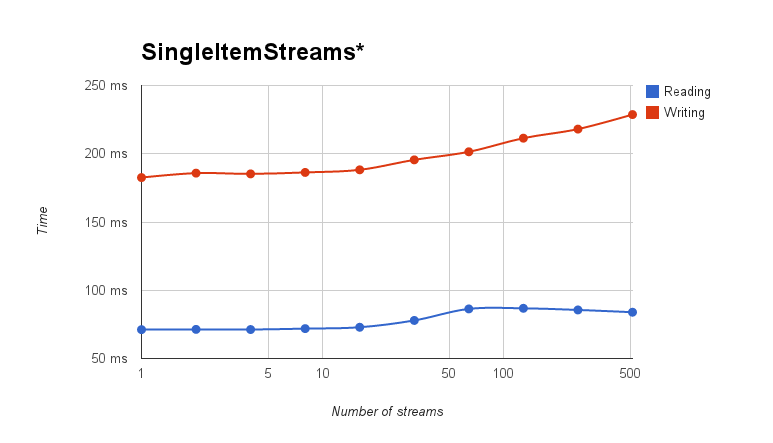
\includegraphics[width=0.5]{SIS.png}
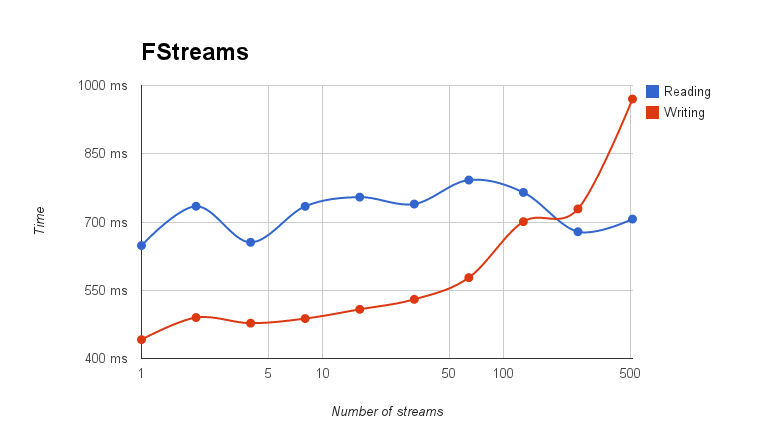
\includegraphics[width=0.5]{FS.png}
The implementation of these streams does not require a manually set buffer size, this is because the OS or the compiler does this in advance. 

The SingleItemStream is behaving as expected; the number of streams does not affect reading very much, and writing increases a bit per stream added, but nothing significant, so it may be attributed to implementation flaws. 

The FStreams graph shows a wide variance in reading, but i stays within a 200ms range not dependant on the amount of streams. Writing on the other hand shows a rapid increase in performance after exceeding 64 streams. 

\subsubsection{BufferedStreams and MMappedStreams}
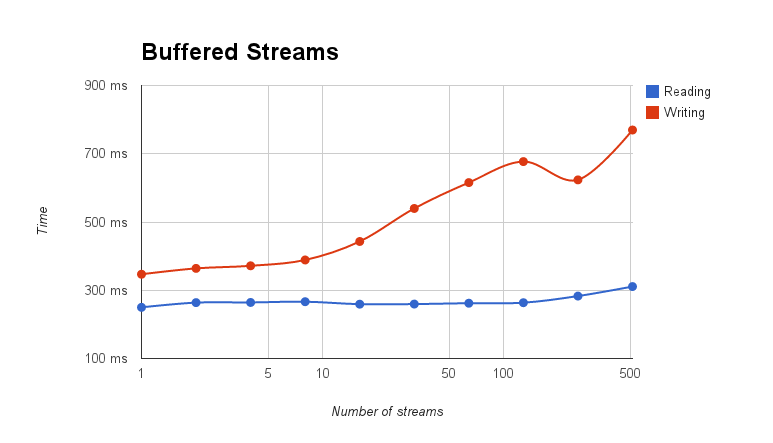
\includegraphics[width=0.5]{BS.png}
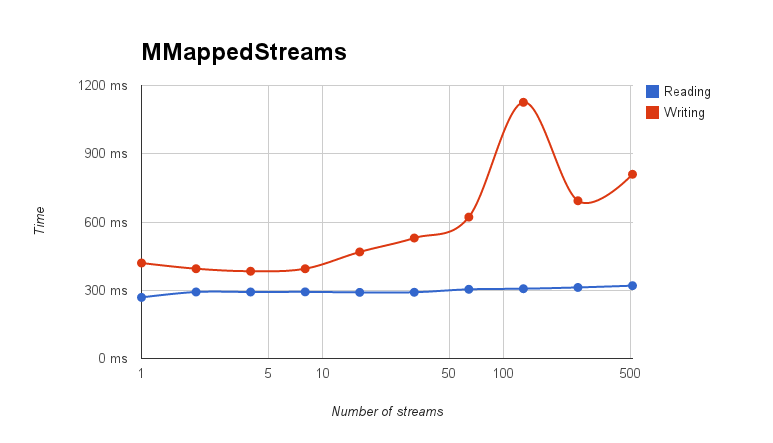
\includegraphics[width=0.5]{MMS.png}
These tests was done with a buffer size of 1024, because this was shown to be the best one when we tested them based on buffersize. 

The BufferedStreams implementation does reading reasonably well, with no significant increase in performance, the writing on the other hand does worse with more streams, with a slight drop around 256 streams, just to continue its performance decline. 

The MMappedStreams behaves similarly to the BufferedStreams, except that the running time is just slightly worse. The running time is practically unchanged for reading, while writing increases in running time the more streams we add. The interesting thing to note here though, is the large decline in performance with a buffer size of 124, afterwards it drops again to expectable levels, and continues as such. 

\subsubsection{Comparing the streams}
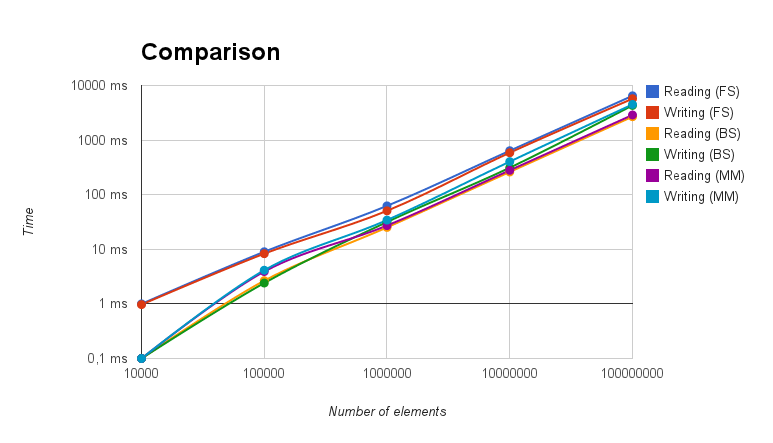
\includegraphics[width=0.5]{parts/StreamCompare.png}
Our comparison graph for the stream implmentaions contain only three of the streams. The single item stream was so slow with large amounts of elements that we did not finish the tests for that implementation. The other streams are closer performance-wise as the graph shows. The streams based on \texttt{fread} and \texttt{fwrite} are clearly slowest which match up with what we expected. Our own buffered implementation slightly outperforms the \texttt{mmap} implementation which is why we ended up chosing that as the streams for our merge sort algorithm.

\subsection{ Finding merge sort parameters}
Andreas

